\begin{frame}{}
  \centering
  {\Large Part I: separating one point from the rest}

  \begin{tikzpicture}
    % \draw (-2, -2) grid (2, 2);
    \node[fill=red, point] at (150:2) {};
    \node[other point] at (30:1) {};
    \node[other point] at (-30:1.5) {};
    \node[other point] at (45:2) {};
    \node[other point] at (-90:0.5) {};

    \draw[thick, gray, dashed] (-1.7, -1.7) -- (.5, 2);
  \end{tikzpicture}
\end{frame}
\begin{frame}{Warm-up}
  \twocols{
    \begin{itemize}
    \item let $x$ be a random point drawn from the equidistribution in the unit ball \nball in \rn
    \item let $0 < r < 1$
    \item let $A=\nball\setminus r\nball$
    \end{itemize}    
  }{
    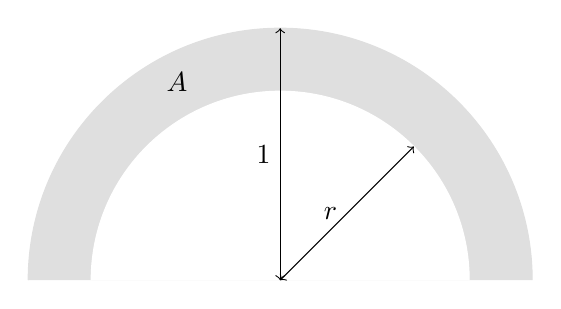
\begin{tikzpicture}[scale=0.8]
      % \draw[step=1cm, gray, very thin] (-4, -4) grid (4, 4);
      \draw[fill, gray!25] (4, -2) arc [start angle=0, end angle=180, radius=4cm];

      \draw[fill, white] (3, -2) arc [start angle=0, end angle=180, radius=3cm];

      \node[] at +(145:2) {$A$};
      \draw[<->] (0, -2) --+(45:3) node [midway, left] {$r$} ;
      \draw[<->] (0, -2) -- +(90:4) node [midway, left] {1} ;
    \end{tikzpicture}    
  }

  \bigskip
  \bigskip
  \[  
     \proba{x \in A} =\; \frac{vol(A)}{vol(\nball)}  =\; 1-r^n
   \]
\end{frame}


\begin{frame}{When is $x$ separable from the rest?}
  \twocols{
    \begin{itemize}
    \item {
        consider a hyperplane $H$ that is
        \begin{itemize}
        \item orthogonal to $x$
        \item and tangent to the inner ball $r \nball$
        \end{itemize}
      }
    \item $\allbutx$ are ``below'' $H$
    \item[] $\rightarrow$ $x$ is separable from $\allbutx$
    \item (the separating hyperplane is $H$)
    \end{itemize}
  }{
    \begin{tikzpicture} [scale=0.8]
      % \draw[step=1cm, gray, very thin] (-4, -4) grid (4, 4);
      \draw (4, -2) arc [start angle=0, end angle=180, radius=4cm];

      \draw (3, -2) arc [start angle=0, end angle=180, radius=3cm];

      \node[] at (0.3, 1.7) {$x$};
      \node[fill=red, point] at (0, 1.7) {};

      \node[other point] at (-2.9, -0.4) {};
      \node[other point] at (-2.8, -1) {};
      \node[other point] at (1.5, -2) {};
      \node[other point] at (2.7, -0.5) {};

      % hyperplane
      \draw (0, -2) -- (0.0, 1.6);
      \pause
      \draw (0, 1) ellipse [x radius=2.55, y radius=0.5];
      \draw[xslant=1.5] (-4.5, 0.25) rectangle (1.5, 2);
      \draw (-2.55, 1) -- (2.55, 1);
      \node at (2, 2.5) {$H$};
    \end{tikzpicture}    
  }
  
  \[\proba{x \text{ is separable from } \allbutx} \ge \proba{\allbutx \text{ are below } H}\]

\end{frame}

\begin{frame}{what is $\proba{\allbutx \text{ are below } H}$?}

  \twocols{
    \begin{itemize}
    \item consider two points, $x$ and $v$
    \item analyze $\proba{v \text{ is above } H}$
    \item {then
        \begin{align*}
        & \proba{\allbutx \text{ are below } H} \\
        =\;& 1-\proba{ \exists v^{'} \in \allbutx \text{ is above } H} \\
        \ge\; &1 - \underbrace{\sum_{v^{'} \in \allbutx} \proba{v^{'} \text{ is above } H}}_{\text{by union bound}}
        \end{align*}

      }
    \end{itemize}
  }{
    \begin{tikzpicture}[scale=0.8]
      % \draw[step=1cm, gray, very thin] (-4, -4) grid (4, 4);
      \draw (4, -2) arc [start angle=0, end angle=180, radius=4cm];
      \draw (3, -2) arc [start angle=0, end angle=180, radius=3cm];


      \node[] at (0.3, 1.7) {$x$};
      \node[fill=red, point] at (0, 1.7) {};
      \node[other point] at (2.4, -0.5) {};
      \node[] at (2.8, -0.5) {$v$};

      \draw (0, 1) ellipse [x radius=2.55, y radius=0.5];

      \node at (2, 2.5) {$H$};      
      \draw (-2.55, 1) -- (2.55, 1);

      % \draw (2.55, 1) arc [start angle=0, end angle=180, radius=2.55cm];
      
      % \draw[<->] (0, -2) --(2.55, 1) node [sloped, midway, below] {1} ;
      % \draw[<->] (0, -2) -- +(90:3) node [sloped, midway, below] {$r$} ;

      % \draw (0cm, 1cm) -- +(2.55, 0) node [sloped, midway, above] {$\sqrt{1-r^2}$} ;
      
    \end{tikzpicture}
  }
\end{frame}

\begin{frame}{Analysis of $\proba{v \text{ is above } H}$}
  \twocols{
    \begin{align*}
      & \proba{v \text{ is above } H} \\
      =\;& \proba{v \text{ lands in  "the cap"}} \\
      =\;& \frac{vol(\text{"the cap"})}{vol(\nball)} \\
      \le \;& \frac{vol(\text{"half the ball"})}{vol(\nball)} \\
      = \;& 0.5 \rho^n
    \end{align*}
    Radius of the ball? $\rightarrow \sqrt{1 - r^2} = \rho$
  }{
    \begin{tikzpicture}[scale=0.8]
      % \draw[step=1cm, gray, very thin] (-4, -4) grid (4, 4);
      \draw (4, -2) arc [start angle=0, end angle=180, radius=4cm];


      \node[] at (0.3, 1.7) {$x$};
      \draw (0, -2) -- (0, 1.7);
      \node[fill=red, point] at (0, 1.7) {};
      
      % \node[other point] at (2.4, -0.5) {};
      % \node[] at (2.8, -0.5) {$v$};

      % \draw[dashed] (2.4, -0.5) -- (0, -0.5);
      % \draw[ultra thick, blue] (0, -2) -- (0, -0.5);


      \only<1>{
        \draw[blue, ultra thick] (0, 1) ellipse [x radius=2.55, y radius=0.5];
        \draw[blue, ultra thick] (2.6, 1) arc [start angle=50, end angle=130, radius=4cm];
      }

      % \node at (2, 2.5) {$H$};

      \uncover<2->{
      % \draw (-2.55, 1) -- (2.55, 1);
      \draw[green, ultra thick] (2.55, 1) arc [start angle=0, end angle=180, radius=2.55cm];
      \draw[green, ultra thick] (0, 1) ellipse [x radius=2.55, y radius=0.5];
      % \draw[<->] (0, -2) --(2.55, 1) node [sloped, midway, below] {1} ;
      % \draw[<->] (0, -2) -- +(90:3) node [sloped, midway, below] {$r$} ;
    }
    \uncover<3->{
      \draw (3, -2) arc [start angle=0, end angle=180, radius=3cm];
      \draw[ultra thick, orange] (0cm, 1cm) -- +(2.55, 0) node [sloped, right] {$\sqrt{1-r^2}$} ;
      \draw[dashed] (0, -2) -- (2.55, 1) node [right, midway] {$1$};
      \draw (0, -2) -- (0, 1) node [right, midway] {$r$};
    }
    \end{tikzpicture}
  }
\end{frame}

\begin{frame}{Putting things together}
  \begin{align*}
    & \proba{x \text{ is separable from } \allbutx} \\
    \ge\;&\proba{x \in A \text{ and } \allbutx \text{ are below } H} \\
    \ge\;& 1 - \underbrace{\proba{x \not\in A}}_{r^n} - \underbrace{\proba{\exists v^{'} \in \allbutx \text{ that is above } H}}_{\le \sum_{v^{'} \in \allbutx} \underbrace{\proba{v^{'} \text{ is above }H}}_{\le \rho^n}} \\
    \ge\; & 1 - r^n - \pr{M-1} \rho^n
  \end{align*}
\end{frame}

\begin{frame}{}
  \begin{center}
    \begin{tikzpicture}
      % \draw[step=1cm, gray, very thin] (-4, -4) grid (4, 4);
      \draw (4, -2) arc [start angle=0, end angle=180, radius=4cm];

      \draw (3, -2) arc [start angle=0, end angle=180, radius=3cm];
      \draw[-Circle] (0, -2) -- (0.1, 1.7) node[xshift=0.2cm] {$x$};  % circle requires loading arrows.meta
      % \node[] at (0.1, 1.7) {$x$};

      \draw (0, 1) ellipse [x radius=2.55, y radius=0.5];

      \draw[xslant=1.5] (-4.5, 0.25) rectangle (1.5, 2);
      \draw (-2.55, 1) -- (2.55, 1);

      % \draw (2.55, 1) arc [start angle=0, end angle=180, radius=2.55cm];
      
      % \draw[<->] (0, -2) --(2.55, 1) node [sloped, midway, below] {1} ;
      % \draw[<->] (0, -2) -- +(90:3) node [sloped, midway, below] {$r$} ;

      % \draw (0cm, 1cm) -- +(2.55, 0) node [sloped, midway, above] {$\sqrt{1-r^2}$} ;
    \end{tikzpicture}
  \end{center}

\end{frame}